
\iffalse
%%%%%%%%%%%%%%%%%%%%%%%%%%%%%%%%%%%%%%%%%%%%%%%%%%%%%%%%%%%%%%%%%%%%%%%%
%
% This is the template file for the 6th International conference
% NONLINEAR ANALYSIS AND EXTREMAL PROBLEMS
% June 25-30, 2018
% Irkutsk, Russia
%
%%%%%%%%%%%%%%%%%%%%%%%%%%%%%%%%%%%%%%%%%%%%%%%%%%%%%%%%%%%%%%%%%%%%%%%%
% The preparation of the article is based on the standard llncs class
% (Lecture Notes in Computer Sciences), which is adjusted with style
% file of the conference.
%
% There are two ways of compilation of the file into PDF
% 1. Use pdfLaTeX (pdflatex), (LaTeX+DVIPS will not work);
% 2. Use LuaLaTeX (XeLaTeX will work too).
% When using LuaLaTeX You will need TTF or OTF CMU fonts
% (Computer Modern Unicode). The fonts are installed with 'cm-unicode' package in
% a distribution of LaTeX % (https://www.ctan.org/tex-archive/fonts/cm-unicode),
% either by downloading and installing these fonts system wide, the address of their page is
% http://canopus.iacp.dvo.ru/%7Epanov/cm-unicode/
% The second option won't work in XeLaTeX.
%
% For MiKTeX (LaTeX distribution for Windows),
%  1. Package 'cm-unicode' is installed manually with the MiKTeX administration Console.
%  2. For the compilation of this example, namely, the stub figure, one will also need to
% download package 'pgf' manually. This package uses in the popular
% package tikz.
%  3. Tests showed that the rest of the required packages MiKTeX loads automatically (if
%     it is allowed). The 'auto download' option is
%     configured in 'Settings' section in MiKTeX Console.
%
%
% The easiest way to compile an article is to use pdfLaTeX, but
% the final layout of the book will be compiled with LuaLaTeX,
% as a result will be of better quality thanks to the package 'microtype' and
% use vector OTF instead of standard raster fonts of pdfLaTeX.
%
% In the case of questions and problems with the article compilation,
% write letters to e-mail: eugeneai@irnok.net, Cherkashin Evgeny.
%
% New version of the correcting style file will be available at the website:
%     https://github.com/eugeneai/nla-style
%     file - nla.sty
%
% Further instructions are in the text body of the template. The template itself
% is an article example.
%
% The LaTeX2e format is used!

% 12 points font size is used.
\documentclass[12pt]{llncs}

% The correcting style file is added.
\usepackage{todonotes}

\usepackage{nla} % This package is needed for compiling
                 % this template, it should be removed
                 % from your article.

% Many popular packages (amsXXX, graphicx, etc.) are already imported in the style file.
% If there is a conflict with your packages, try disabling them and compile
% the text.
%
% It would be convenient in the layout of the proceedings if the file names
% of the figures of different authors do not clash.
% To minimize the clash, the drawings can be placed in a separate subfolder
% named after the author or the title of the paper.
%
% \graphicspath{{ivanov-petrov-pics/}} % specifies the folder with images in png, pdf formats.
% or
% \graphicspath{{great-problem-solving-paper-pics/}}.

\begin{document}

% Text should be formatted in accordance with the 'article' class, using extensions like
% AMS.
%

\fi


\title{Transmissionless propagation of the kink soliton for the nonlinear klein-gordon equation on branched structures}
% First author
\author{Quvonchbek Asadov\inst{1} \and  Karimjon Sabirov\inst{2,3}
}
\institute{University of management and future technology, Tashkent, Uzbekistan\\
  \email{quvonchbekurinovichasadov@gmail.com}
  \and
EMU University, Tashkent, Uzbekistan;\\
$^3$ Tashkent university of information technologies, Tashkent, Uzbekistan\\
\email{karimjonsabirov80@gmail.com}}
% etc

\maketitle

\begin{abstract}

In this paper we consider the nonlinear Klein-Gordon equation on
the metric star graph with three semi-infinite bonds. At the
branched point we put two types of vertex boundary conditions: the
weight continuity and the condition for derivatives of wave
functions as the generalized Kirchhoff rule. We solve this
equation satisfying vertex boundary conditions. We also show reflectionsless
propagations of the kink soliton solution.


\keywords{nonlinear Klein-Gordon equation, vertex boundary conditions, generalized Kirchhoff rule, reflectionsless transmission, kink soliton, metric graphs.}
\end{abstract}

% at the end of the list, there should be no final dot

\section{Introduction and formulation of the problem}

In this work we focus on one of the exact solutions and
transmission of the kink soliton of the nonlinear Klein-Gordon
equation \cite{Book1} through the vertices of the networks \cite{Book2} -\cite{Article5}.

We consider a star graph shown Fig.1 with three bonds $e_j$, for which a
coordinate $x_j$ is assigned. Choosing the origin of coordinates
at the vertex, 0, for bond $e_1$ we put $x_1\in(-\infty,0]$ and
for $e_{2,3}$ we fix $x_{2,3}\in[0,+\infty)$. In what follows, we use the shorthand notation $q_{j}(x)$ for $q_j(x_j)$ where $x$ is the coordinate on the bond $j$ to which the component $q_j$ refers. Klein-Gordon equation on the each bond $e_j$ of the star graph is written as

\begin{equation}
\partial_{tt}^2 q_j - \partial_{xx}^2 q_j - q_j + b_{j} q_{j}^3 =
0.\label{kgeq1}
\end{equation}

% The figures and tables are drawn according to the standard class 'article'.
\begin{figure}[htb]
  \centering

% Two picture formats are supported:
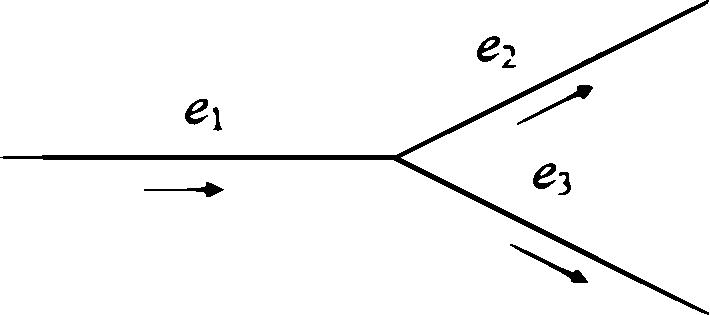
\includegraphics[width=0.5\linewidth]{StarGraph.pdf} % Raster format
%\includegraphics[width=0.7\linewidth]{figure.png} % Vector and raster format
%
% Vector drawings can be drawn in Inkscape editor
% https://inkscape.org/ru/download/
% The usual format of the editor is SVG, so the drawings must be exported in
% PDF or PNG (with a resolution of minimum 150 dpi, and maximum of 300 dpi).
%  \begin{center}    \missingfigure[figwidth=0.7\linewidth] \end{center}
  \caption{The metric star graph}\label{pic1}
\end{figure}

Now we define the vertex boundary conditions at the branched point
of the star graph, therefore we derive these boundary conditions
from conservation laws. One of the conservation laws is energy defined as

\begin{equation}
E = \sum_{j=1}^3 E_j,\label{conl1}
\end{equation}
where

\begin{equation}
E_j= \int _{e_j} \left[ \frac{1}{2} (\partial_t q_j)^2 +
\frac{1}{2} (\partial_x q_j)^2 - \frac{1}{2} q_j^2 + \frac{b_j}{4}
q_j^4 \right] dx.\label{energy1}
\end{equation}

From $\dot{E}=0$ we can get the following nonlinear boundary
condition as

\begin{equation}
\partial_x q_1 \partial_t q_1 |_{x=0} = \partial_x q_2 \partial_t q_2 |_{x=0} + \partial_x q_3 \partial_t q_3|_{x=0}.\label{nbc1}
\end{equation}

We need two types of boundary conditions to find a solution of
(\ref{kgeq1}) and to fulfil the nonlinear vertex boundary
condition (\ref{nbc1}). Therefore the first type of vertex
boundary conditions is the following weight continuity

\begin{equation}
 \alpha_1 q_1 |_{x=0}= \alpha_2 q_2 |_{x=0} = \alpha_3 q_3 |_{x=0},\label{wc1}
\end{equation}
the second type of vertex boundary conditions is given derivatives of wave functions at the branched point as Kirchhoff rule

\begin{equation}
 \frac{1}{\alpha_1} \partial_x q_1 |_{x=0} = \frac{1}{\alpha_2} \partial_x q_2 |_{x=0} + \frac{1}{\alpha_3} \partial_x q_3 |_{x=0}.\label{kr1}
\end{equation}

\section{The kink soliton solution of Klain-Gordon equation on the star graph with three edges}

The kink (antikink) soliton solution of Klein-Gordon equation
(\ref{kgeq1}) on the each bond $e_j$ of the metric star graph is
the following

\begin{equation}
 q_j (x,t) = \mp \frac{1}{\sqrt{b_j}} \, {\rm tanh} \left( \frac{x - l - \upsilon t}
{\sqrt{2(1 - \upsilon^2) }} \right),\label{sol1}
\end{equation}
where $l$ is the initial center of mass of soliton (the kink and
antikink soliton solutions are with the signs $-$ and $+$,
respectively). Fulfilling the vertex boundary conditions
(\ref{wc1})-(\ref{kr1}) we can get the following constrains

\begin{eqnarray}
\frac {\alpha_1}{\sqrt{b_1}} = \frac {\alpha_2}{\sqrt{b_2}} =
\frac{\alpha_3}{\sqrt{b_3}},\label{const1}\\
\frac {1}{\alpha_1 \sqrt{b_1}} = \frac {1}{\alpha_2 \sqrt{b_2}} +
\frac{1}{\alpha_3 \sqrt{b_3}}.\label{const2}
\end{eqnarray}

From Eq.s(\ref{const1}) and (\ref{const2}) we obtain the following sum rule for nonlinearities

\begin{equation}
\frac {1}{b_1} = \frac {1}{b_2} + \frac {1}{b_3}.\label{sr1}
\end{equation}


Using the kink (antikink) soliton solution of Klein-Gordon
equation (\ref{kgeq1}) with the sum rule for the nonlinearities
(\ref{sr1}) we can also show that the momentum is conserved.

\section{Conclusion}

In this work we studied the nonlinear Klein-Gordon equation on
the simplest metric graphs as the star graph with three
semi-infinite bonds. From the weight continuity and the condition for derivatives of the wave function as Kirchhoff rule we obtained nonlinear boundary conditions at the vertex (branched point) derived from the energy conservation law. We obtained the soliton solution on the metric star graph and the constrain as inverses of nonlinearities for the reflectionless transmission. We can also extend obtained results to other topologies such as tree and loop graphs.


% At the end of the text, acknowledgments are expressed, if you haven't
% made a footnote from the title. For example, we can write

\begin{thebibliography}{9} % or {99}, if there is more than ten references.

\bibitem{Book1} Ablowitz M.J., Segur H. Solitons and the Inverse Scattering Transform. Philadelphia, 1981.

\bibitem{Book2} Ablowitz M.J., Clarkson P.A. Solitons, Nonlinear Evolution Equations and Inverse Scattering. London, Cambridge University Press, 1991.

\bibitem{Proceedings1} Greiner W. Relativistic Quantum Mechanics-Wave Equations. Springer-Verlag, 3rd~ed. Berlin, 2000.

\bibitem{Article1} Ablowitz M.J., Kruskal M.D. and Ladik J.F. Solitary wave collisions. SIAM J. Appl. Math.~1979. Vol.~36, no~3. Pp.~428--437.

\bibitem{Article2} Jim´enez S., V´azquez L. Analysis of Four Numerical Schemes for a Nonlinear Klein-Gordon Equation. J. Appl. Math. 1990. Vol.35, Issue 1. Pp.~61--94.

\bibitem{Article22} Los Vu-Quos, Shaofan Li. Invariant-conserving finite difference algorithms for the nonlinear Klein-Gordon equation. J. Comp. Meth. in App. Mech. and Eng. (North-Holland, CMA 403), 1993. Vol. 107. Pp.~341--391.

\bibitem{Article3} Sabirov K.K., Babajanov D.B., Matrasulov D.U. and Kevrekidis P.G. Dynamics of dirac solitons in networks. J. Phys. A: Math. Theor.~2018. Vol.~51. P.~435203.

\bibitem{Article4} Sabirov K.K., Yusupov J.R., Matyokubov Kh.Sh., Susanto H., Matrasulov D.U. Networks with point-like nonlinearities. J. Nanosystems: Phys. Chem. Math.~2022. Vol.~13, no~1. P.~3035.

\bibitem{Article5} Yusupov J.R., Sabirov K.K., Asadov Q.U., Ehrhardt M., and Matrasulov D.U. Dirac particles in transparent quantum graphs: Tunable transport of relativistic quasiparticles in branched structures. J. Phys. Rev. E.~2020. Vol.~101. P.~062208.      
\end{thebibliography}
%\end{document}

%%% Local Variables:
%%% mode: latex
%%% TeX-master: t
%%% End:
